\documentclass{article}
\usepackage{parskip}
\usepackage{pdfpages}
\usepackage[margin=.6in]{geometry}
\begin{document}
\includepdf[pages=2]{slides}
There is time asymetry with how energy works. For instance dropping an egg can only go one direction.

\includepdf[pages=3]{slides}
We start with a hot up of coffee with lots of thermal energy. We leave it to sit for a while and it starts passing its thermal energy to the air around it. So we have concentrated energy spontaneously disperse, but we never see the opposite happen. This is called entropy.

\includepdf[pages=4-5]{slides}
Brownian motion was used as proof fro democratus's ideas.

\includepdf[pages=7]{slides}
Diffusion is the migration of particles from high concentration to a region of low concentration. This happens randomly without outside influence.

\includepdf[pages=8]{slides}
All motion is random. So we look at the average particles. Say we divide some water into cross sections. We can say that on average half of the particles in one section will move right and half will move left. This results in this diffusion of particles from high to low concentration. From this we can derive a law which is boss.

\includepdf[pages=9]{slides}
The end result of diffusion is a dynamic equilibrium because shits still moving but a balance has been reached.

\includepdf[pages=10]{slides}
Nature does not prefer an spread out of dye molcules in water. It really doesn't care. Its basically just a probabilty thing. There are way more possibilities that have more spread out particles rather than clumps.

\includepdf[pages=11]{slides}
There si random jiggling of water molecules which is held over from the big band theory. These water molecules collide with the dye molecules. These move things around. Statistically speaking it is nearly guarenteed that the mixture will end up looking homogeneous.

Our body is very good at extracting order from the things we consume. So basically we are reversing the diffusion process.

\includepdf[pages=12]{slides}
The diffusion process defined above also applies to the energy in a coffee cup. We call this law of diffusion the second law of thermal dynamics.

\includepdf[pages=13]{slides}
Basically the second law of thermal dynamics is that energy tends to spread out. Entropy is kind of a measure of disorder. It is possible to have places in the universe where entropy is decreasing, but you will always have a net positive growth of entropy.

What animates us is random thermal motion left over from the big bang which our body extracts order from and uses to move.

\includepdf[pages=14]{slides}
\includepdf[pages=15]{slides}
Entropy was first denoted with S. It stated around the time people wanted to make steam engines more efficient. The energy flowing from the hot object to the cold object divided by the temperature. Doing this for the hot object and the cold object are not equal (they sum to a non zero value). When you add them you get a positive value. This means that the cold object has more entropy.

This lead us to know that the amount of entropy is always increasing.

\includepdf[pages=16]{slides}
The equation $S=k\log W$ gives us a great understanding of entropy.

\includepdf[pages=17]{slides}
A water droplet has a fairly high level of disorder (many ways to arrange them and have it look the same), but when we freeze it there is much less disorder (fewer ways for it to be arrange).

\includepdf[pages=18]{slides}
Crystal structures have some order, but you can rearrange them alot. But if you try to do the same with dna lots of shit changes. So we can say that dna is highly ordered.

\includepdf[pages=19]{slides}
$S=k\log W$

K is Boltzmann's constant. For the sake of understanding we are just going to ignore this, its a constant, who cares. W is the number of microstates compatible with a given macrostate.

\includepdf[pages=20]{slides}
Take a balloon for example. We can describe its macrostate using a few parameters (volume, temperature, pressure). The microstate however is determined on the position, and velocity of every air molecule.

\includepdf[pages=21-29]{slides}
There is a point at which the temperature of the system is the same as its environment. At this point equilibrium has been reached. No more diffusion then.

\includepdf[pages=30-41]{slides}
Theres an argument that life violates the second law of thermal dynamics because entropy goes down in cells. This is actually fine, there is nothing that says entropy can never go down, just that its net is increasing. Similar arguments are made for evolution which is dumb.

Yeah, at this point I totally stopped paying attention. He just sorta continued rambling on about how entropy works. You got this future lara, I believe in you.

Shame on you past Lara, you fucked up. But not as badly as Steven when he typed that.
\includepdf[pages=42-31]{slides}
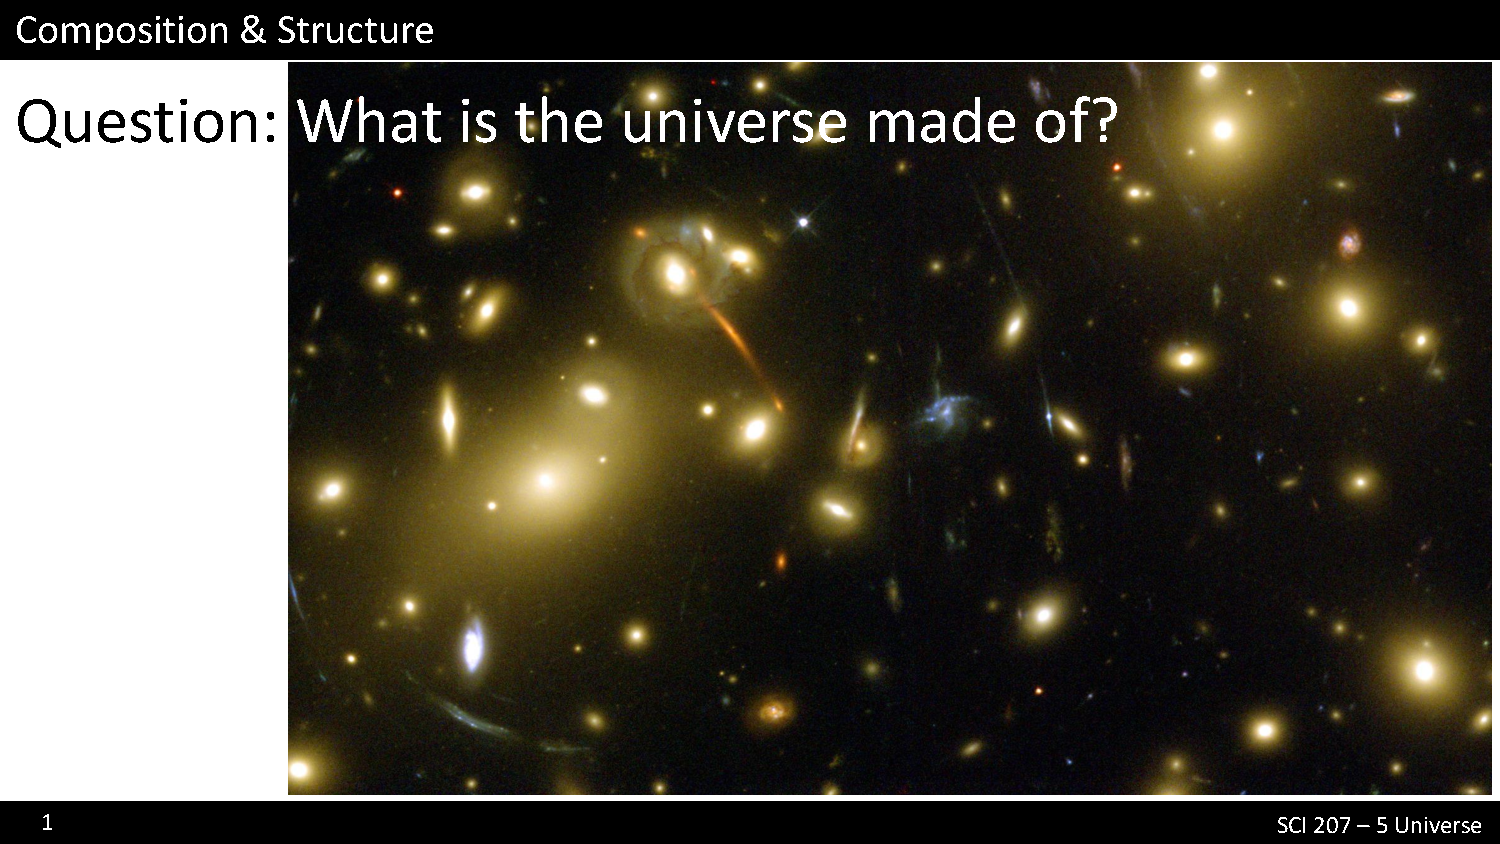
\includepdf[pages=1-33]{slides2}
Light energy is highly ordered, when plants process it they make glucose which is less ordered. We burn that chemical energy and turn it into kinetic/thermal energy which is highly unordered. We have this molecule adp which has only two phosphate groups, meaning its in its low energy state. We use energy to attach another phosphate making it atp, the high energy state. This is used all over the fucking place in our body.

\includepdf[pages=34-37]{slides2}
By providing the elections with a very specific path to go through (the copper wire). This is how we make a battery. Like the piston this is a one way valve.

\includepdf[pages=38-40]{slides2}
The election flow does directly charge the conversion to atp. Instead it drives a protein pump. The elections pump out proteins from the cell. There is a valve called atp synthase. It opens to allow adp into it and when a proton is pushed out the adp converts into atp.

\includepdf[pages=41-42]{slides2}
The conversion of adp to atp acually happens due to the mitochondria. Its hella complicated. Watch the video.

\includepdf[pages=43-44]{slides2}
The proton pump moved a bunch of ions on one side of the cell membrane. They want to come back in but the cell wall stops them. The valve opens when the cell needs energy to allow some protons back in. The protons rush in and turn a wheel (an actual wheel). The wheel has some adp on it and it slams it into a phosphate group clicking them together. You can even run the motor in reverse. Its boss.

\includepdf[pages=45-48]{slides2}
The universal battery that powers all life is this action of creating a proton gradient and using it with atp sythase. Because all life uses this its clear that its a clue to the origin of all life.

\includepdf[pages=49]{slides2}
\includepdf[pages=50]{slides2}
We need proteins to create a proton gradient but the way we build proteins uses energy that we get from atp which requires a protein gradient. So where did the original energy come from to create the first proteins, the spark of life so to speak.

Fairly recently we realized that if you look at hydrothermal vents you can find naturally occurring proton gradients. These can just randomly synthesize things. The theory is that the rocks around the vents ``came to life''.

\includepdf[pages=51]{slides2}
There are two groups for theories of life. One is self replication first (RNA world). The other is metabolism first (deep sea hydrothermal vents).

\includepdf[pages=52-55]{slides2}
Basically we are taking our models and making them more and more probable. It is unlikely that we will ever find definitive proof since almost everything around at the beginning of life have been subducted into the earths course.


Well thats the end of the slides on learn, but not his slides. WEEEEEE.

Thermodynamics is the study of a closed system near equilibrium, but life needs things to be out of wack to work

Dissipative structures were disovered by Progoine. When they are open they have energy flowing through them. This results in a steady state not equilibrium which is basically ordered energy. When you start with a low energy system and add heat to it we get convection cells, called Benard cells. These appear spontaneously. This decreases entropy because it brings order. These also carry energy through much more quickly. This could be considered analagous to a living system.

With this logic we can see that it is possible to have a system be continuously out of equilibrium, so long as we have energy going it we can maintain our weird state.

If you have tons of little things interacting with each other we can have self-organizing systems. This is basically order occuring spontaneously which is neat. An example of this is the formation of cell membranes.

We have expanded our understanding of the second law of thermaldynamics by understanding that withing microscopic system we can have a fluctuating entropy. This is the fluctuation theorem. In small fluctuations the probability of it being increasing is equivalent to it decreasing. In large fluctuations its more probable to be increasing.

\begin{equation}
	\frac{P(+\Delta S)}{P(-\Delta S)} = e^{\Delta S}
\end{equation}

We then expanded more and more on this by creating a generalized theorem and then getting that to apply it to life.

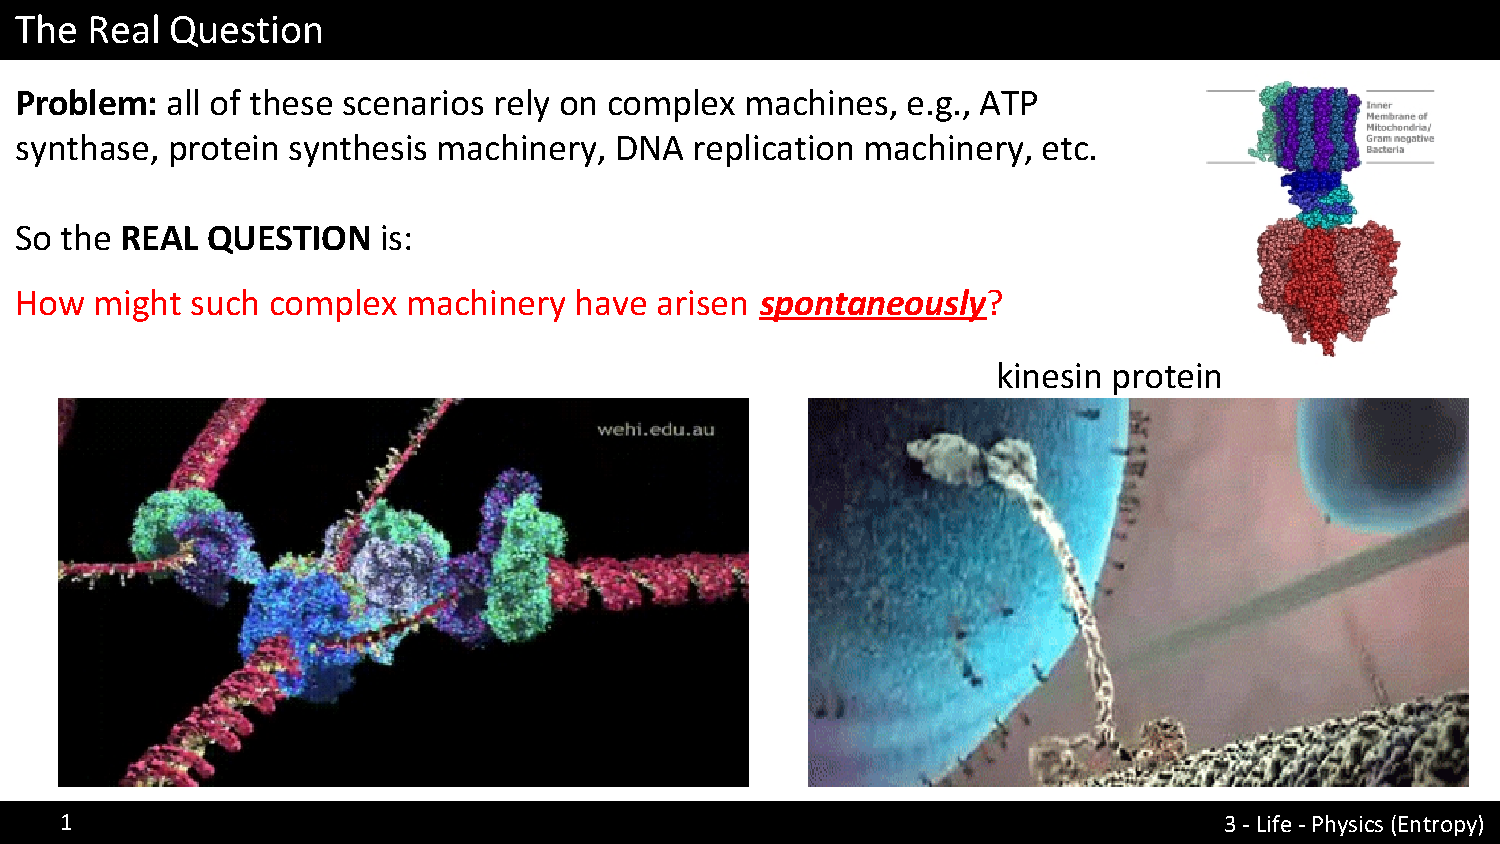
\includepdf[pages=1-16]{slides3}
Basically we are explaining why things that are based on thermaldynamics want to replicate. This ties physics to biology.

\includepdf[pages=17]{slides3}
Clumps of atoms in a bath at some temperature (the water molecules are moving very fast with thermal energy). Any life molecule is being struck millions of times violently from every direction by water molecules. Overtime the atoms will rearrange themselves to ressonate better with the forces acting on them. AAAAAHHHHHHH CAPS LOCK NOOOOOOO

fuck you steven

\includepdf[pages=18-20]{slides3}
So you have these atoms in a bath being jostled, this jostling is not enough to break atomic bonds. When you get an external force (like the sun, or deep sea vents) the jostling becomes enough to make atomic changes. So we are making these atomic changes at moments when the atom is particularly susceptible to it. This makes the atom more able to obsorbe energy so they are less likely to fall apart. This results is entropy moving in one direction more and more.

\includepdf[pages=21-24]{slides3}
We think that if we shine light on water these structures could spontaneously occur to obsorb the light. An experiment was done with silver nano rods and showed that the rings would spontaneously form rings that can absorb sunlight.

\includepdf[pages=25-27]{slides3}
If we liken this to darwinian evolution its adaptation without replication. Here we just have shit randomly adapting to their environment.

\includepdf[pages=28]{slides3}
Replication is a great method of dissipation. We can also conclude that life emerging randomly is not only possible but highly probable.

\includepdf[pages=29]{slides3}
Votices just use free energy. They just straight increase entropy in the universe. They also replicate, those fuckers, increasing the growth of entropy.

\includepdf[pages=30-40]{slides3}





















\end{document}
